\section{Tahapan Desain}
\label{sec:tahapan-desain}
\begin{figure}[htbp]
    \centering
    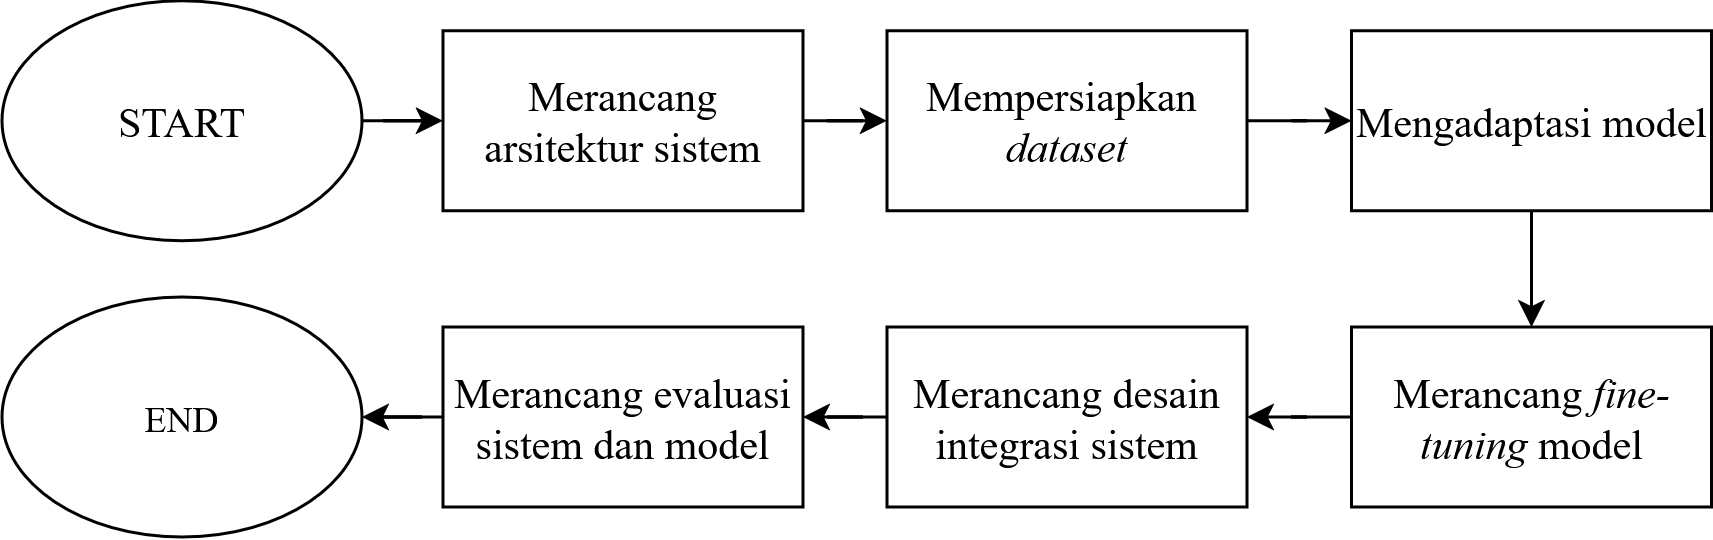
\includegraphics[width=\textwidth]{images/design-flow.png}
    \caption{Alur kerja tahapan desain sistem ekstraksi data struk dan bukti pembayaran}
    \label{fig:design-flow}
\end{figure}

\autoref{fig:design-flow} menunjukkan tahapan desain yang dilakukan dalam penelitian ini. Tahapan desain utama mencakup perancangan \emph{fine-tuning} model, perancangan konversi model, perancangan aplikasi \emph{mobile}, dan perancangan \emph{backend service}. Tahapan desain yang dihasilkan akan menjadi dasar untuk mengembangkan sistem ekstraksi data struk dan bukti pembayaran. Tahapan desain dirancang berdasarkan pada alternatif solusi yang telah diusulkan pada \autoref{sec:analisis-pemilihan-solusi} dan disesuaikan dengan tahap desain pada metodologi \dsrm.

\subsection{Analisis Kebutuhan dan Arsitektur Sistem}
\label{subsec:analisis-kebutuhan-arsitektur}

Tahapan pertama dalam perancangan sistem adalah melakukan analisis kebutuhan dan merancang arsitektur sistem yang sesuai dengan tujuan penelitian. Berdasarkan analisis kebutuhan yang telah dilakukan pada \autoref{sec:analisis-kebutuhan}, sistem dirancang untuk memenuhi kebutuhan fungsional dan non-fungsional yang telah didefinisikan.

Arsitektur sistem dirancang menggunakan pendekatan \textit{client-server} dengan pemisahan yang jelas antara aplikasi \textit{mobile} sebagai \textit{frontend} dan layanan \textit{backend} untuk pemrosesan model. Keputusan untuk menggunakan arsitektur terdistribusi ini didasarkan pada kompleksitas model \donut{} yang memerlukan sumber daya komputasi tinggi dan tidak dapat dijalankan secara efisien pada perangkat \textit{mobile}.

% \begin{figure}[htbp]
%     \centering
%     \includegraphics[width=0.9\textwidth]{images/system-architecture.png}
%     \caption{Arsitektur sistem ekstraksi data pembayaran}
%     \label{fig:system-architecture}
% \end{figure}

\autoref{fig:system-architecture} menunjukkan arsitektur sistem yang terdiri dari tiga komponen utama: aplikasi \textit{mobile}, layanan API, dan modul pemrosesan model. Aplikasi \textit{mobile} berfungsi sebagai antarmuka pengguna untuk mengambil gambar, menampilkan hasil ekstraksi, dan mengelola data transaksi. Layanan API berperan sebagai penghubung antara aplikasi \textit{mobile} dan modul pemrosesan model, menangani \textit{request} dari klien dan mengembalikan hasil dalam format yang terstruktur.

Modul pemrosesan model mengimplementasikan dua model \donut{} yang berbeda: model \textit{QRIS-TF} untuk ekstraksi dan klasifikasi bukti pembayaran digital, dan model \textit{CORD-v2} untuk ekstraksi data dari struk pembayaran berbasis kertas. Pemilihan model dilakukan secara otomatis berdasarkan jenis dokumen yang diproses, memastikan setiap dokumen ditangani oleh model yang paling sesuai.

Arsitektur ini memberikan fleksibilitas dalam pengembangan dan pemeliharaan sistem, memungkinkan peningkatan model atau penambahan fitur baru tanpa mempengaruhi komponen lain. Selain itu, pendekatan terdistribusi memungkinkan sistem untuk menangani beban pemrosesan yang besar dan dapat diskalakan sesuai kebutuhan.


